\section{System Overview and Threat Model}
\label{sec:system_threat}

This section establishes the operating principles of the Truth Beam recording system, states precisely the threat model under which its verifier is evaluated, enumerates the trust assumptions, and defines what ``verification'' means in this work. The aim is to fix the scope of every claim that follows, so that the quantitative results in later sections are read against a clearly bounded adversary and a clearly bounded notion of authenticity.

\subsection{System overview: a chain-coupled projector--camera loop}
\label{sec:system_threat:overview}

The Truth Beam is a tamper-evident video-recording system built around a closed projector--camera feedback loop. At each chain step $t$ a \SI{32}{\byte} chain state $S_t$ is deterministically expanded, per channel and with domain separation, by a BLAKE3 extendable-output function (BLAKE3-XOF)~\cite{blake3} into a structured-light emission tile $E_t$. The tile is a $1080\times1920$ RGB, \SI{8}{bit}-per-channel fractional-Brownian-motion (fBm) field: each per-channel \SI{32}{\byte} seed is XOF-expanded to \num{43110} bytes and decomposed into four octaves on grids $(17,30),(34,60),(68,120),(135,240)$, then composited by bit-exact integer bilinear upsampling and integer accumulation to a final \texttt{uint8} tile. $E_t$ is projected onto the scene by a $1920\times1080$ projector (with an exemplary refresh on the order of \SI{16}{\milli\second} per the patent~\cite{patent2025}), and the illuminated scene is photographed by a camera built around a Sony IMX540 sensor (The Imaging Source) configured to deliver \SI{8}{bit} BayerRG8. Each raw capture $C_t$ is exactly \num{24472000} bytes at shape $(4600,5320)$ with an RGGB color-filter array, demosaiced through OpenCV's \texttt{COLOR\_BayerBG2RGB\_EA} flag. The entire loop is \SI{8}{bit} end-to-end: XOF bytes, emission PNGs, and BayerRG8 capture all live in $[0,255]$; the IMX540's native \SI{12}{bit} ADC notwithstanding, no part of the loop operates above \SI{8}{bit}.

The feedback that gives the system its tamper-evidence is the fold-back step. The raw Bayer bytes of $C_t$ are hashed ($\texttt{bayer\_blake3} = \mathrm{BLAKE3}(C_t)$, \SI{32}{\byte} output), and this hash---together with a \SI{28}{\byte} capture-meta struct and a drand~\cite{drandbeacon} quicknet beacon (an \SI{8}{\byte} big-endian round number and \SI{32}{\byte} round randomness)---is folded into the next state $S_{t+1}$ through a domain-separated BLAKE3 transition. The emission committed at row $t$ is in turn derived from that same row's state $S_t$, i.e.\ $E_t = \mathrm{gen}(\mathrm{XOF}(S_t))$ ($\texttt{target\_chain\_row} = \texttt{capture\_row} = t$; see \Cref{subsec:pc_offset}). The loop therefore closes: substituting any capture $C'_t \neq C_t$ yields a different \texttt{bayer\_hash}, hence a different next state $S_{t+1}$, hence a different downstream emission $E_{t+1}$, and the divergence is detectable by any party holding a sample of the chain. (A shifted $+1$ alignment is used by some verification-side probes, discussed in \Cref{subsec:pc_offset}; the empirically optimal verifier offset is unmeasured, but the recording convention itself --- $E_t$ from $S_t$ --- is unambiguous.)

The system was exercised in two same-rig recording sessions of a single human performer, which supply all data used in this report. Session D2 (\texttt{cittadel\_first\_human}, \num{5992} chain rows) was recorded under the v9 chain ($\texttt{ROW\_DOMAIN\_TAG} = \texttt{b"TB:ROW:v9"}$); session V10 (\texttt{cittadel\_v10\_mainnet\_improv}, \num{3743} rows) under the v10 chain ($\texttt{b"TB:ROW:v10"}$), which additionally folds a \SI{32}{\byte} \texttt{ai\_payload\_root} committing AI-agent response frames. The protocol versions are structurally distinct in their per-row transition, so v9 logs cannot be re-walked under v10; this is the substrate for the same-rig cross-protocol observations reported later (\Cref{sec:results_main_generalization}).

\Cref{fig:overview} shows the per-frame decision the system poses: given a raw capture $C$ and the emission $E$ that the chain prescribes for it, is $C$ consistent with the recorded chain-coupled illumination?

\begin{figure}[t]
\centering
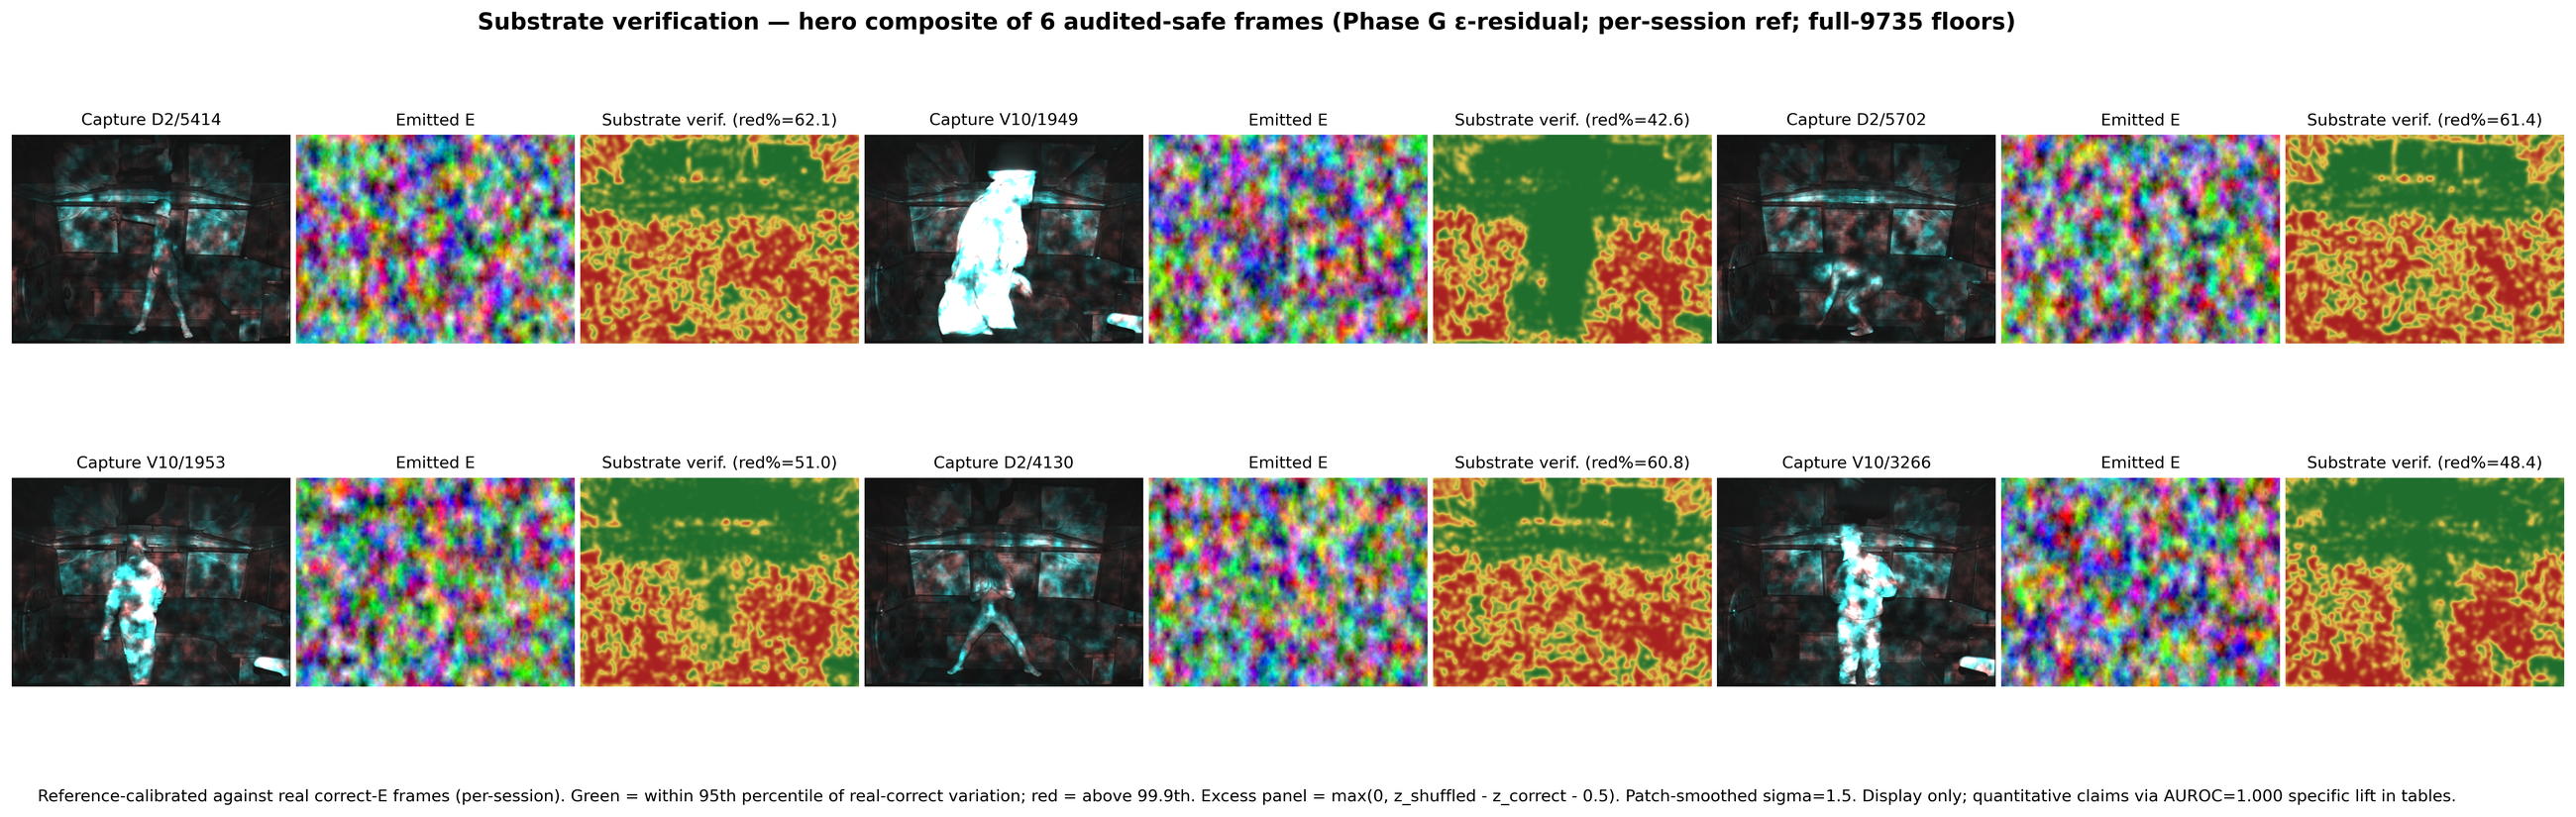
\includegraphics[width=\linewidth]{figures/fig_overview.png}
\caption{System overview and per-frame decision. Six audited-safe high-signal captures (three D2 yoga, three V10), each shown as a triple: the raw camera capture $C$, the emitted chain-coupled pattern $E$ that was projected, and the substrate-verification residual map. The verification map answers one question per frame---is this capture consistent with the recorded chain-coupled emission? Green indicates consistency; red indicates an anomalous (un-coupled) region. Calibrated against real-correct $E$ frames per session; green where the robust $z$ lies below threshold, red above; the excess panel is $z_{\mathrm{two}}$ minus the per-pixel p99.9 floor at margin~0.5; $\sigma=0.0$ (paper detail). Frames are drawn from the \num{9733} body-safe pool ($\text{body\_red} < 0.5\%$); no manual body suppression is applied.}
\label{fig:overview}
\end{figure}

\subsection{What a verifier observes}
\label{sec:system_threat:observable}

The property that makes verification possible is that a genuine recording carries a learnable \emph{physical coupling} between $C_t$ and $E_t$. The projector emits a chain-derived fBm field; the camera records the scene under that field as a raw BayerRG8 frame; and the optical channel imposes a characteristic relationship between the two. This coupling is what the verifier learns to recognize. A useful empirical anchor for what survives the optical channel is an early single-session (D2) characterization: emission RGB structure can be recovered from raw capture at validation PSNR $\approx \SI{26.20}{\decibel}$, whereas direct per-cell XOF byte prediction sits at chance (validation bit accuracy $=0.500$). In other words, the channel acts as an optical low-pass: the coupling that survives to the camera is emission-RGB-style structure, not byte-level XOF detail. This distinction matters for the threat model below, because it bounds which substitutions are optically detectable.

\subsection{Threat model}
\label{sec:system_threat:threat}

The adversary's goal is singular: to have a recording \emph{accepted as authentic} when it is not. Concretely, the adversary wants a verifier to certify a capture as a genuine, chain-coupled photograph of the real scene under the prescribed emission. Two attack avenues realize this goal.

\paragraph{Forge-under-known-$E_{\mathrm{target}}$.} The adversary knows the target emission $E_{\mathrm{target}}$ (it is chain-derived and, in our evaluation, treated as known to the attacker) and synthesizes a fake capture $C_{\mathrm{fake}}$ intended to pass as a genuine capture of the scene under $E_{\mathrm{target}}$. To succeed, $C_{\mathrm{fake}}$ must simultaneously (i)~reproduce the physical coupling that a real capture exhibits with respect to $E_{\mathrm{target}}$ and (ii)~be a realistic raw BayerRG8 capture in its own right. The concrete instantiation of this attacker used throughout this work is the learned editor F-A v1: a \num{42.3}-million-parameter ControlNet-style~\cite{zhang2023controlnet} editor that produces $C_{\mathrm{fake}}$ conditioned on $E_{\mathrm{target}}$ together with source-capture and source-emission hints.

\paragraph{Tamper.} The adversary modifies a genuine recording---substituting, editing, or re-ordering captured frames---while attempting to keep the chain self-consistent. Because the captured bytes are hashed into the next state, any such substitution propagates: a changed $C_t$ implies a changed $S_{t+1}$ and hence a changed expected $E_{t+1}$, so a tampered segment can be exposed by re-walking the chain against a held reference. This is the protocol-level (cryptographic) line of defense and is distinct from the learned verifier; the two are complementary.

\paragraph{Within-attack contrasts used for evaluation.} Beyond a wholesale fake, we evaluate finer substitutions that probe \emph{which} part of the coupling a verifier relies on: pairing a real capture with a temporally mis-aligned or shuffled emission (wrong-$E$), substituting emissions across octaves or channels, and applying fine XOF-level bit-flips to the emission. These are diagnostic perturbations of the emission side of the $(C,E)$ pair rather than full forgeries, and they let us characterize the verifier's sensitivity profile (\Cref{sec:redteam_item1}).

\subsection{Trust assumptions}
\label{sec:system_threat:trust}

The verifier's guarantees are conditioned on the following assumptions.

\begin{itemize}
  \item \textbf{Holder of a chain sample.} Tamper-evidence requires that the verifier (or auditor) holds a trustworthy sample of the chain---at minimum the recorded chain states and capture hashes---against which to check consistency. The closed-loop argument is meaningless to a party that holds neither the chain nor a reference.
  \item \textbf{Honest recording-time hashing and beacon handling.} The protocol assumes the recorder folds the true captured bytes, capture-meta, and a locally verified drand signature into the transition. The chain transition itself does not re-verify the drand signature; a sentinel (round number $0$, value all-zeros) is folded verbatim when the beacon is unavailable, and the verifier notes \texttt{drand\_availability} as \textsc{partial} or \textsc{missing} without gating the pass/fail decision on it.
  \item \textbf{Genuine captures carry learnable coupling.} The learned verifier assumes that real $(C_t, E_t)$ pairs from the operating rig exhibit a consistent physical coupling that fakes and mispairings violate; this is an empirical property of the optical channel established on the two sessions studied here.
  \item \textbf{Known target emission.} The forging adversary is assumed to know $E_{\mathrm{target}}$. This is the strong, conservative assumption: it grants the attacker the very signal the verifier checks against, so success under it is a meaningful test of coupling fidelity rather than of emission secrecy.
\end{itemize}

\subsection{What ``verification'' means here}
\label{sec:system_threat:verification}

Verification in this work is a per-frame consistency test, not an identity, semantic, or content-authenticity judgment. The verifier scores a single $(C_t, E_t)$ pair and asks whether $C_t$ is consistent with the chain-coupled emission $E_t$; it does not attempt to recover the XOF bytes, nor to assert anything about the scene's meaning. The learned instantiation (Phase~G, detailed in \Cref{sec:verifier_method}) is a diffusion-residual scorer: a capture is deemed typical when the noise-prediction residual $\lVert \hat{\epsilon}-\epsilon\rVert^2$ is small for the recorded emission and anomalous when it is large, with the emission entering as a conditioning hint rather than as a denoising target.

Two scope guards bound every claim in this report and are stated here once, to be carried throughout.

\begin{itemize}
  \item \textbf{Same-rig scope.} All results are obtained on a single physical rig across two recording sessions (D2 and V10) of one performer. Generalization claims are \emph{same-rig cross-session} (and, where v9 and v10 are both involved, \emph{same-rig cross-protocol}) only. Nothing here establishes cross-rig, cross-camera, cross-projector, or cross-subject generalization.
  \item \textbf{Attacker scope.} The evaluated forging adversary is F-A v1. A stronger adaptive attacker, F-A v2, exists only as a design specification: it is \emph{not trained} and its trainer code does not exist. Accordingly, this work makes \emph{no} claim of robustness against a strong or adaptive attacker; such robustness is explicitly future work (\Cref{sec:results_redteam}).
\end{itemize}

With the system, the adversary, the trust assumptions, and the meaning of verification fixed, the remainder of the report develops the verifier architecture, its quantitative separability against F-A v1, the localization of the discriminative signal, and the sensitivity of the verifier to graded emission perturbations.
